% ---------------------------------------------------------------------
% EG author guidelines plus sample file for EG publication using LaTeX2e input
% D.Fellner, v2.01, Oct 06, 2016


\title[Interactive Point Set Joint Registration and Co-segmentation]%
{Interactive Point Set Joint Registration and Co-segmentation}

% for anonymous conference submission please enter your SUBMISSION ID
% instead of the author's name (and leave the affiliation blank) !!
\author[Paper 1049]
{\parbox{\textwidth}{\centering Paper 1049}
	\\
	% For Computer Graphics Forum: Please use the abbreviation of your first name.
	{\parbox{\textwidth}{\centering  
			%        $^2$ Another Department to illustrate the use in papers from authors
			%             with different affiliations
		} 
	}
}
% ------------------------------------------------------------------------

% if the Editors-in-Chief have given you the data, you may uncomment
% the following five lines and insert it here
%
% \volume{27}   % the volume in which the issue will be published;
% \issue{1}     % the issue number of the publication
% \pStartPage{1}      % set starting page


%-------------------------------------------------------------------------
\begin{document}
	
	\teaser{
		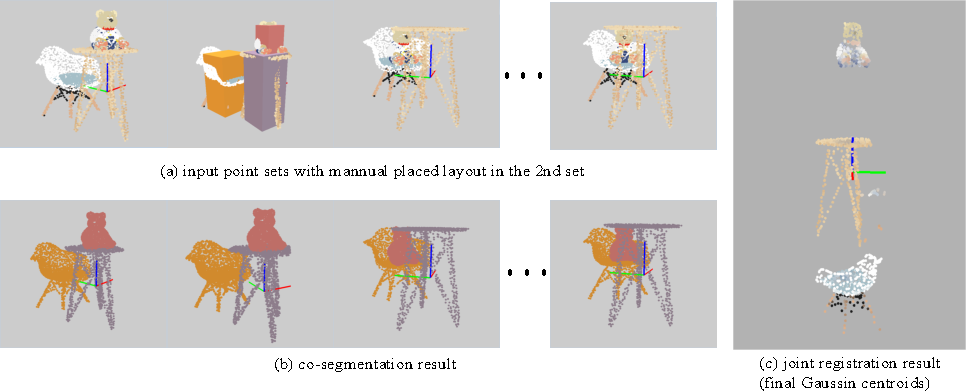
\includegraphics[width=0.8\linewidth]{images/teaser/teaser2}
		\centering
		\caption{Given a series of point sets and user-placed object layout boxes in one point set (a), our method jointly segment and register objects in the point sets to generate object-level co-segmentation (b) and registration to object models represented as GMM (c).}
		\label{fig:teaser}
	}
	
	\maketitle
	
	\begin{abstract}
		We present a novel approach of joint registration and co-segmentation for point sets where objects move in different ways. 
		Considering the joint registration and co-segmentation as two problems heavily entangled with each other, we represent the input point sets as samples from a generative model and bring up with a novel formulation based on Gaussian mixture model. %
		By maximizing the posterior probability of the samples, we gradually recover the latent object models as well as an object-level segmentation, and simultaneously align the segmented points to the latent object models. 
		%
		Along with the formulation, we design an interactive tool that helps users intuitively intervene the process to optimize the registration and segmentation result. 
		%
		The experiment results on a group of synthetic and scanned point clouds demonstrate that our method is powerful and effective for joint registration and co-segmentation on point sets of multiple objects.  
		
		\begin{classification} % according to http:http://www.acm.org/about/class/1998
			\CCScat{COMPUTER GRAPHICS}{I.3.8}{Applications}
			\CCScat{IMAGE PROCESSING AND COMPUTER VISION}{I.4.8}{Scene Analysis}{Range data}
		\end{classification}
		
	\end{abstract}
	
	
	%-------------------------------------------------------------------------
	\section{Introduction}
\label{sec:intro}
In many researches and applications of indoor scenes the data of segmented and even annotated 3D indoor scenes are required as either data base or training data (e.g.\cite{SceneFromExample}\cite{Fisher:2012:ESO:2366145.2366154}\cite{Chen:2014:ASM:2661229.2661239}\cite{Fisher:ActivityCentricSceneSynthesis}).\\
One way to build such data base is to interactively compose scenes from 3D shape models resulting in scenes with object segmentation and annotation naturally available, or to mannually segment and annotate existing scenes. This procedure can be tedious and time consuming, despite the efforts to improve the interaction experience(e.g.\cite{Merrell:2011:IFL:2010324.1964982}\cite{Xu:2013:SSC:2461912.2461968}).\\
Another way is to automatically generate scenes from 3D shape models according to the input RGB or RGB-D images(e.g.\cite{Liu2015Model}\cite{Chen:2014:ASM:2661229.2661239}). In such methods, a retrievial procedure is usually needed and inevitablely limit the result to a certain set of 3D models despite the actual 3D model in the input images.\\
We prefer a approach that helps us build such data set directly from the captured data. One of the major gap between the required data set and available scene capturing framework(e.g.\cite{KinectFusion}) is the general object level segmentation. We want to stress that a general object level segmentation problem should not be treated as an equivalence of multilabel classification problem since it is not limited to a certain set of objects. For 3D data, \cite{3DReasoningfromBlockstoStability} used some simplified physical prior knowledge (i.e. the block based stability) to help acheiving the general object segmentation, while the work of \cite{Xu:2015:ACS:2816795.2818075} proposes a practical and rather complete framework to close the gap between the required data set and available scene capturing method. One of the observation in \cite{Xu:2015:ACS:2816795.2818075} is that the motion consistency of rigid object can serve as a strong evidence of general objectness. To exploit this fact, they employ a robot to do proactive push and use the movement tracking to verify and iteratively improve their object level segmentation result. Our work presented in this paper is trying to exploit the same observation from a different approach.\\
We intend to use the motion consistency that is naturally revealed by human activities along the time. Down to this approach, we are facing the choice of scanning scheme. One way is to record the change of the scene along with the human activities, another is to arrange a daily or even a once every half day sweep to only record the result of human activities but avoid the instant of human motion. The main challenge brought in by the second scheme is that we may not be able to solve the object correspondence by a local search due to the sparse sampling over time, but the very same challenge exists in the first scheme due to the exclusion caused by human bodies not to mention other additional process(e.g. tracking with severe oclussion ) needed for human bodies. With the second scanning scheme, our original intention of building 3D scene data set from capturing naturally leads us to the problem of coupled joint registration and co-segmentation.\\ In this problem, registration and segmentaion are entangled in each other. On one hand the segmentation depends on the registration to connect the point clouds into series of rigid movement so that the object level segmentation can be done based on the motion consistency, on the other hand, the registration depends on the segmentation to break the problem into a series of rigid joint registration instead of a joint registration with non-coherent point drift(A pair of points is close to each other in one point set but their correspondent pair of points in another point set is far from each other, in other words, the point drift of this pair is non-coherent. This happens when this pair of points actually belong to different objects.)\\
To model the problem, we employ a group of gaussian mixture models and each of these gaussian mixture models represents a potential objects. This modeling handles the entanglement of registration and segmentation in the way that      
      
	\section{Related Work}
\label{sec:rw}
\subsection{Point Set Registration with GMM Representation}
\cite{TPS_RPM}\\
\cite{CPD}\\
\cite{GMM_PAMI}\\
Our work is most related to \cite{Evangelidis2014}. We actually extend the formulation of \cite{Evangelidis2014} to simultaneously handle joint registration and co-segmentation.
\subsection{Functional Mapping}
The coupled joint registration and co-segmentation problem comes with a latent problem of point-to-point correspondence problem. A series of work based on the functional maps representation advocated in \cite{Ovsjanikov:2012:FMF:2185520.2185526} have be done. In one of the most recent work \cite{Maron:2016:ConvRelax}, a convex relaxation technique was used to better approximate the global minimal for both rigid and non-rigid registration problem. 

\subsection{Primitive Fitting} 
\cite{GlobFit2011} 
	\section{Method Overview}
\label{sec:method}
\subsection{Problem Statement}
Given $M$ point sets with $I_m$ points $V_m=\{\pmb{v}_{mi}\}$ for the $m^{th}$ point set (Figure \ref{fig:teaser} (a) shows an example of input point sets.), we intend to simutaneously partition the point sets into $N$ objects and find the rigid transformations $\{\phi_{mn}(\pmb{x})=R_{mn}\pmb{x}+\pmb{t}_{mn}\}$ that transform each object model to its observed position in each input point set.  For partition, we output point-wise label vectors $\{\pmb y_m\}$ for each input point set to indicate its object partition. ( Figure~\ref{fig:teaser} (b) illustrates result label vectors by assigning same color to points with same label. ) To establish our formulation, we first summarize the symbols that will be used as in Table \ref{tab:symbol}.
\begin{table}[!hbp]
\centering
\begin{tabular}{c l}
\hline
Symbol & Meaning\\
\hline
$V$ & The input point sets.\\
$V_m$ & The $m^{th}$ input point set.\\
$\pmb v_{mi}$ & The $i^{th}$ point of $V_m$.\\
$\pmb f_{mi}$ & The point-wise feature vector of $\pmb v_{mi}$.\\
$z_{mi}$ & The latent parameter for $\pmb v_{mi}$.\\
& $z_{mi}=k$ means $v_{mi}$ is generated by $k^{th}$ Gaussian\\
$Z$ & $Z=\{z_{mi}|m=1...M,i=1...I_m\}$\\
$K_{all}$ & The total number of Gaussian models.\\
$K_n$   & The number of Gaussian for $n^{th}$ object. $\sum_n^N K_n = K_{all}$\\
$p_k$  & The weight of $k^{th}$ Gaussian. $\sum_k^{K_{all}}p_k=1$\\
$\pmb x_k$ & The centroid of $k^{th}$ Gaussian.\\
$\pmb {xv}_k$ & The centroid of $k^{th}$ Gaussian for point position.\\
$\pmb {xf}_k$ & The centroid of $k^{th}$ Gaussian for point feature.\\
$\Sigma_k$ & The covariance matrix of $k^{th}$ Gaussian.\\
$\sigma_k$ & $\Sigma_k=\sigma_k^2I$. ($I$ is identity matrix here.)\\
$\sigma v_k$ & Gaussian covariance parameter for point position\\
$\sigma f_k$ & Gaussian covariance parameter for point feature\\
$\phi_{mn}$ & Transformation from $n^{th}$ object to $m^{th}$ input set.\\
$R_{mn}$ & The rotation matrix for $\phi_{mn}$.\\
$\pmb t_{mn}$ & The translation vector for $\phi_{mn}$.
\end{tabular}
\caption{Table of Symbols Used in the Paper}
\label{tab:symbol}
\end{table}
\subsection{Basic Formulation}

To simutaneously model the joint registration and co-segmentation,  we come up with a generative model as follows:
\begin{equation}
\label{equ:model}
P(\pmb{v}_{mi})=\sum^{K_n}_{k=1}p_k\mathcal{N}(\pmb{v}_{mi}|\phi_{mn}(\pmb{x}_k),\Sigma_k)
\end{equation}
which treat the $i^{th}$ observed point $v_{mi}$ from the $m^{th}$ point set as a sample point generated by one of $N$ object models.
Each object model is represented by a group of $K_n$ gaussian models.\\
The model parameters are:
$$\Theta=\{\{p_k,\pmb x_k,\Sigma_k\}_{k=1}^{\sum{K_n}},\{\phi_{mn}\}_{m=1,n=1}^{MN}\}$$
The problem is how to estimate the parameters for the model to fit all the input point sets. The problem can be solved within the framework of expectation maximization. In particular, we bring in a latent parameter as:\\
$$Z=\{z_{mi}|m=1...M,n=1...I_m\}$$
such that $z_{mi}=k(k=1,2...,K_{all})$ assigns the observed point $v_{mi}$ to the $k^{th}$ component of Gaussian mixture model. We aim to maximize the expected complete-data log-likelihood:
\begin{equation}
\label{equ:obj0}
\varepsilon(\Theta|V,Z)=\mathbb{E}_Z[\ln P(V,Z;\Theta)|V]={\sum_ZP(Z|V,\Theta)\ln{P(V,Z;\Theta)}}
\end{equation}
Such formulation can be seen as an adaption of joint registration formulation in \cite{Evangelidis2014}, upon which we seperate Gaussian models into groups to express multiple objects and the latent parameter  $Z$ that assign observed points to gaussian models can naturally indicate the object level segmentation.\\
By the asssumption of independent and identically distributed of input points, we can rewrite the objective (\ref{equ:obj0}) into:
\begin{equation}
\label{equ:obj2}
\Theta=\arg\max\sum_{mik}\alpha_{mik}(\ln p_k + \ln P(\pmb v_{mi}|z_{mi}=k;\Theta))
\end{equation}
where $\alpha_{mik} = P( z_{mi} = k | \pmb v_{mi} ; \Theta )$\\
By bringing in equation \ref{equ:model} and ingnoring constant terms, we can rewrite the objective as:
\begin{equation}
\label{equ:obj3}
\Theta=\arg\max\sum_{mik}\alpha_{mik}(||\pmb v_{mi}-\phi_{mn}(\pmb x_k)||_{\Sigma_k}^2 + \ln |\Sigma_k| - 2\ln p_k)
\end{equation}
where the $|\cdot|$ denotes the determinant and $||x||_A^2=x^TA^{-1}x$. It is predefined that $x_k$ is one of the gaussian centroid used to represent $n^{th}$ object, which is why we apply transformation $\phi_{mn}$ on to the $x_k$. For the convenience of computation, we restrict the model to isotropic covariances, i.e.,$\Sigma_k=\sigma^2I$ and $I$ is the identity matrix.\\
Now, we can optimize this through iterating between estimating $\alpha_{mik}$ (Expectation-step) and maximizing $f(\Theta|V,Z)$ sequentially with respect to each parameters in $\Theta$ (Maximization-steps).
These steps are:\\
\textbf{E-step}:
this step estimates the posterior probability $\alpha_{mik}$ of $v_{mi}$ to be a point generated by the $k^{th}$ Gaussian model.\\
\begin{equation}
\label{equ:estep}
\alpha_{mik}=\frac{p_k\sigma_k^{-3}exp(-\frac{1}{2\sigma_k^2}||v_{mi}-\phi_{mn}(\pmb x_k)||^2)}{\sum_s^{K_{all}}p_s\sigma_s^{-3}exp(-\frac{1}{2\sigma_s^2}||v_{mi}-\phi_{mn}(\pmb x_s)||^2)}
\end{equation}
\textbf{M-step-a}:this step update the transformations $\phi_{mn}$ that maximize $f(\Theta)$, given instant values for $\alpha_{mik}$, $x_k$, $\sigma_k$. We only consider rigid transformations, making  $\phi_{mn}(x)=R_{mn}x+t_{mn}$. The maximizer $R_{mn}^*,t_{mn}^*$  of $f(\Theta)$ is the same with the minimizers of the following constrained optimization problems:\\
\begin{equation}
\left\{
\begin{array}{rcl}
\min_{R_{mn},t_{mn}}&      &||(W_{mn}-R_{mn}X_n-\pmb t_{mn}\mathbf{e}^T)\Lambda_{mn}||_F^2\\
s.t.&      &R_{mn}^TR_{mn}=I, |R_{mn}|=1\\
\end{array} \right.
\end{equation}
where $\Lambda_{mn}$ is $K_n \times K_n$ diagonal matrix with elements $\lambda_{mnk}=\frac{1}{\sigma_k}\sqrt{\sum_i^{I_{m}}\alpha_{mik}}$,$I_m$ is the number of point for the $m^{th}$ input point set, $X_n = [\pmb x_1, \pmb x_2,...., \pmb x_{K_n}]$ is the matrix stacked by the centroids of gaussian models that are predefined to represent the $n^{th}$ object. $\mathbf{e}^T$ is a vector of ones, $||\cdot||_F$ denotes the Frobenius norm, and $W_{mn}=[w_{m1},w_{m2},...,w_{mk},...,w_{mK_n}]$, in which $w_{mk}$ is a weighted point as:\\
\begin{equation}
w_{mk}=\frac{\sum_{i=1}^{I_m}\alpha_{mik} \pmb v_{mi}}{\sum_{i=1}^{I_m}\alpha_{mik}}
\end{equation}
This problem have a similar solution of in \cite{Evangelidis2014}. The only difference is that we are estimating the transformation from Gaussian models to the input point sets instead of the transformation from input point sets to Gaussian models, since there are multiple group of $\pmb x_k$ corresponding to multiple objects in our Gaussian models. The optimal can be given by:\\
\begin{equation}
\label{equ:updateR}
R_{mn}^*=U_{mn}C_{mn}V_{mn}^T
\end{equation}
\begin{equation}
\label{equ:updatet}
t_{mn}^*=\frac{1}{tr(\Lambda_{mn}^2)}(W_{mn}-R_{mn}X_n)\Lambda_{mn}^2\mathbf{e}
\end{equation}
where $[U_{mn},S,V_{mn}]=svd( W_{mn}\Lambda_{mn}P_{mn}\Lambda_{mn}X_{mn}^T )$ and $P_{mn}=I-\frac{\Lambda_{mn}\mathbf{e}(\Lambda_{mn}\mathbf{e})^T}{(\Lambda_{mn}\mathbf{e})^T\Lambda_{mn}\mathbf{e}}$,$I$ is identity matrix. $C_{mn}=diag(1,1,|U_{mn}||V_{mn}|)$.\\
\textbf{M-step-b}: this step we update the parameters related to the Gaussian mixture model and the indicating vector for object segmentation 
\begin{equation}
\label{equ:updatexk}
\pmb x_k^*=\frac{\sum_{m=1}^M\sum_{i=1}^{I_m}\alpha_{mik}(R_{mn}^{-1}v_{mi}-\pmb t_{mn})}{\sum_{m=1}^M\sum_{i=1}^{I_m}\alpha_{mik}}
\end{equation}
where $\pmb x_k$ is one of the Gaussian centroids that is predefined to represent $n^{th}$ object. 
\begin{equation}
\label{equ:updatesigma}
\sigma_k^{*2}=\frac{\sum_{m=1}^M\sum_{i=1}^{I_m}\alpha_{mik}||(v_{mi}-\pmb t_{mn}-R_{mn}^*\pmb x_k^*)||_2^2}{3\sum_{m=1}^M\sum_{i=1}^{I_m}\alpha_{mik}}
\end{equation}
\begin{equation}
\label{equ:updatepk}
p_k^*=\frac{\sum_{m,i}\alpha_{mik}}{M}
\end{equation}
\begin{equation}
\label{equ:updatey}
y_{m}(i)^*=\arg \max_n \sum_{k=K_{n-1}+1}^{K_n} \alpha_{mik} 
\end{equation}
where $y_{m}(i)$ is the $i^{th}$ entry of the indicate vector $y_m$.
\subsection{Bilateral Formulation}
When considering point-wise features, we can add bilateral terms into the generative model.
\begin{equation}
P(v_{mi},f_{mi})=\sum^{K_n}_{k=1}p_k\mathcal{N}(v_{mi}|\phi_{mn}(\pmb{xv}_k),\sigma v_k)\mathcal{N}(f_{mi}|\pmb{xf}_k,\sigma f_k)
\end{equation}
where $f_{mi}$ is the feature vector for point $v_{mi}$ and $xf_k$ is the feature vector for $k^{th}$ point in latent model. As shown in the formulation, there is no transformation applyed onto $xf_k$, which means that this formulation is only suitable to the features that is rotation and translation invariant. For example, the point color vector(for all the result in this paper we use RGB color as feature vector ) $[red_{mi},green_{mi},blue_{mi}]$ is a suitable feature for this formulation.In this formulation $N(v_{mi}|\phi_{mn}(xv_k),\sigma v_k)$ is the spatial term and $N(f_{mi}|xf_k,\sigma f_k)$ is the feature term.
For the bilateral formulation, iteration steps will be as follows:\\
\textbf{E-step}:in this step the calculation of posterior probability need to consider both the spatial term and the feature term.
\begin{equation}
\label{equ:bestep}
\alpha_{mik}=\frac{p_kP_v(v_{mi},\phi_{mn}(xv_k),\sigma v_k)P_f(f_{mi},xf_k,\sigma f_k)}{\sum_s^{K_{all}}p_sP_v(v_{mi},\phi_{mn}(xv_s),\sigma v_s)P_f(f_{mi},xf_k,\sigma f_s)}
\end{equation}
where $P_v(x,y,\sigma)=\sigma^{-3}exp(-\frac{1}{2\sigma^2}||x-y||^2)$ and $P_f(x,y,\sigma)=\sigma^{-D(x)}exp(-\frac{1}{2\sigma^2}||x-y||^2)$ and $D(x)$ means the dimension of the vector $x$.\\
\textbf{M-step-a:}for bilateral formulation, this step is the same with the basic formulation and the update can be done as (\ref{equ:updateR}) and (\ref{equ:updatet}).
\textbf{M-step-b}:for bilateral formulation, this step need not only update model centroids and variance for spatial term as (\ref{equ:updatexk}) and (\ref{equ:updatesigma}).
but also update the centroids and variance for feature term as in (\ref{equ:updatefk}) and (\ref{equ:updatefsigma})\\
\begin{equation}
\label{equ:updatefk}
xf_k^*=\frac{\sum_{m=1}^M\sum_{i=1}^{I_m}\alpha_{mik}f_{mi}}{\sum_{m=1}^M\sum_{i=1}^{I_m}\alpha_{mik}}
\end{equation}
\begin{equation}
\label{equ:updatefsigma}
\sigma f_k^{*2}=\frac{\sum_{m=1}^M\sum_{i=1}^{I_m}\alpha_{mik}||(f_{mi}-xf_k^*)||_2^2}{D(f)\sum_{m=1}^M\sum_{i=1}^{I_m}\alpha_{mik}}
\end{equation}
where $D(f)$ is the dimenssion of feature vectors.\\
The update of $p_k$ for bialateral formulation is the same as the basic formulation in (\ref{equ:updatepk}).
\subsection{Interaction Design}
\label{sec:imp:interact}
Unfortunately, there are a large number of parameters that can not be easily initialized in our formulation . In this subsection we first introduce our design of interaction, which is intuitive for users to input the semantic prior this way. We then explain how we can easily initlialize those parameters for our optimization based on the manual input.\\
As demonstrated in Figure~\ref{fig:interact}, we let user choose one of the point sets and placing and editing boxes in it to indicate the layout for this point set. From this, we can easily initialize the total number of objects $N$ and determine $\{K_n\}$ which is the numbers of Gaussian mixture models used to represent each object.
\begin{figure}[htb]
	\centering
	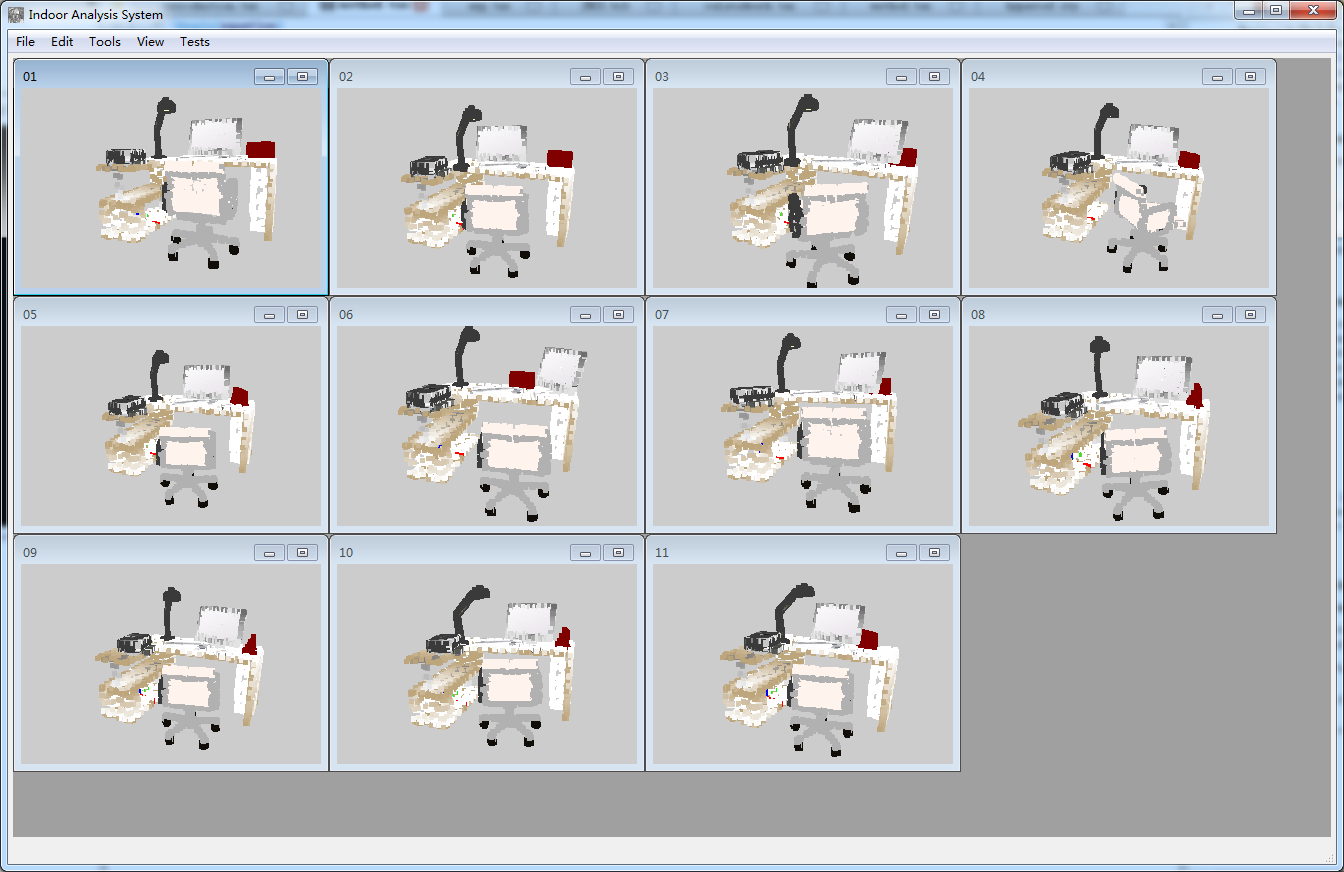
\includegraphics[width=.3\linewidth]{images/interact01.png}
	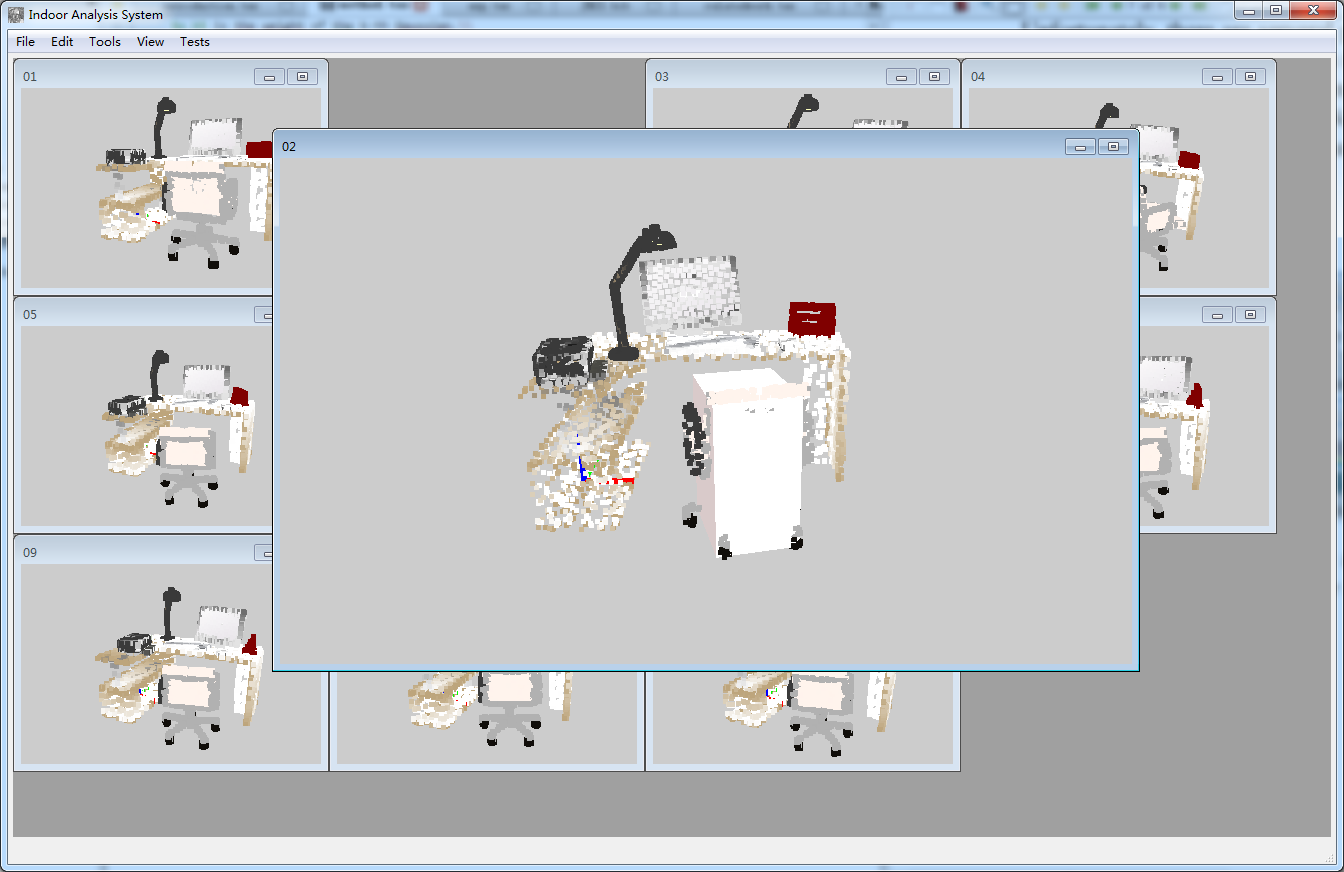
\includegraphics[width=.3\linewidth]{images/interact02.png}
	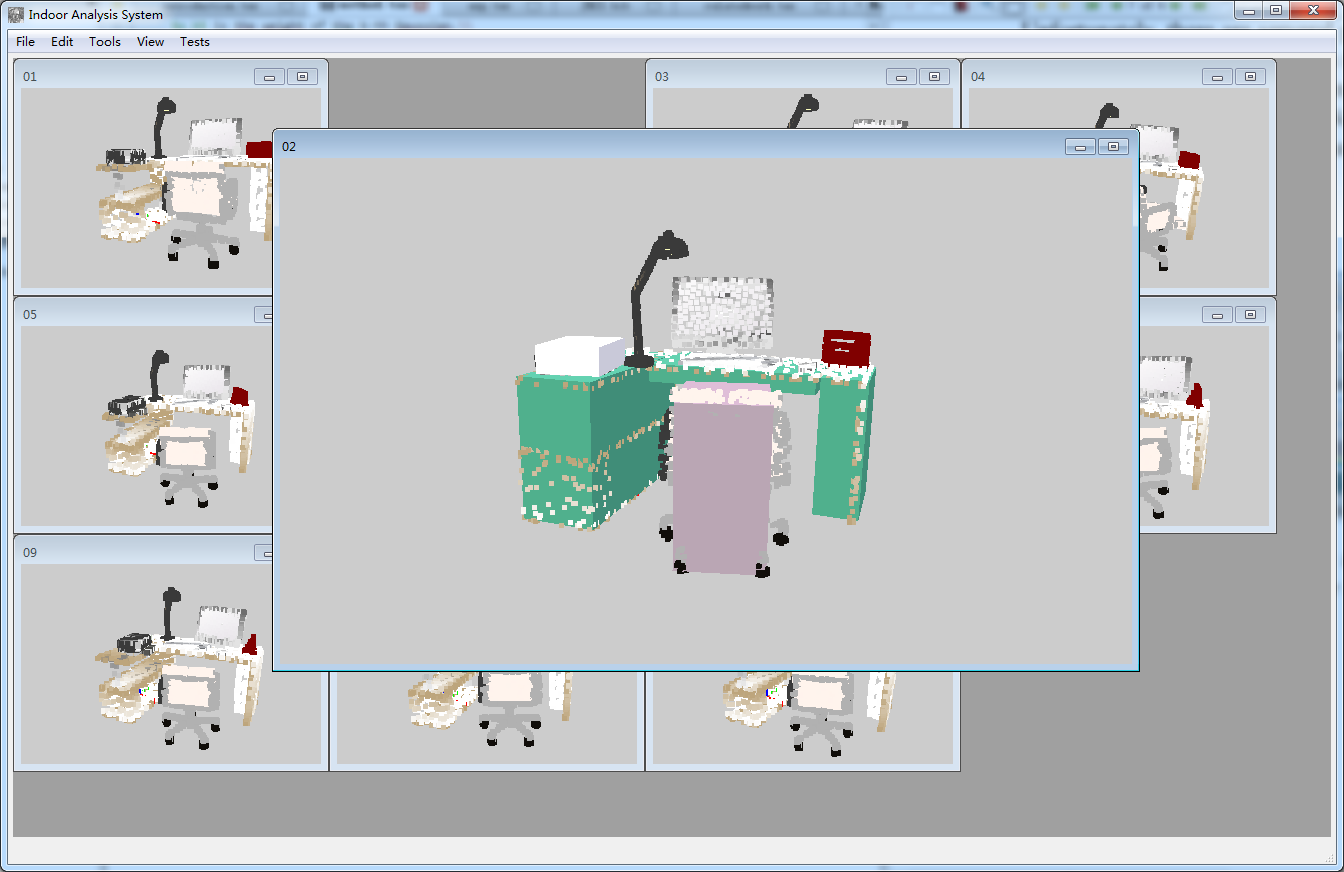
\includegraphics[width=.3\linewidth]{images/interact03.png}
	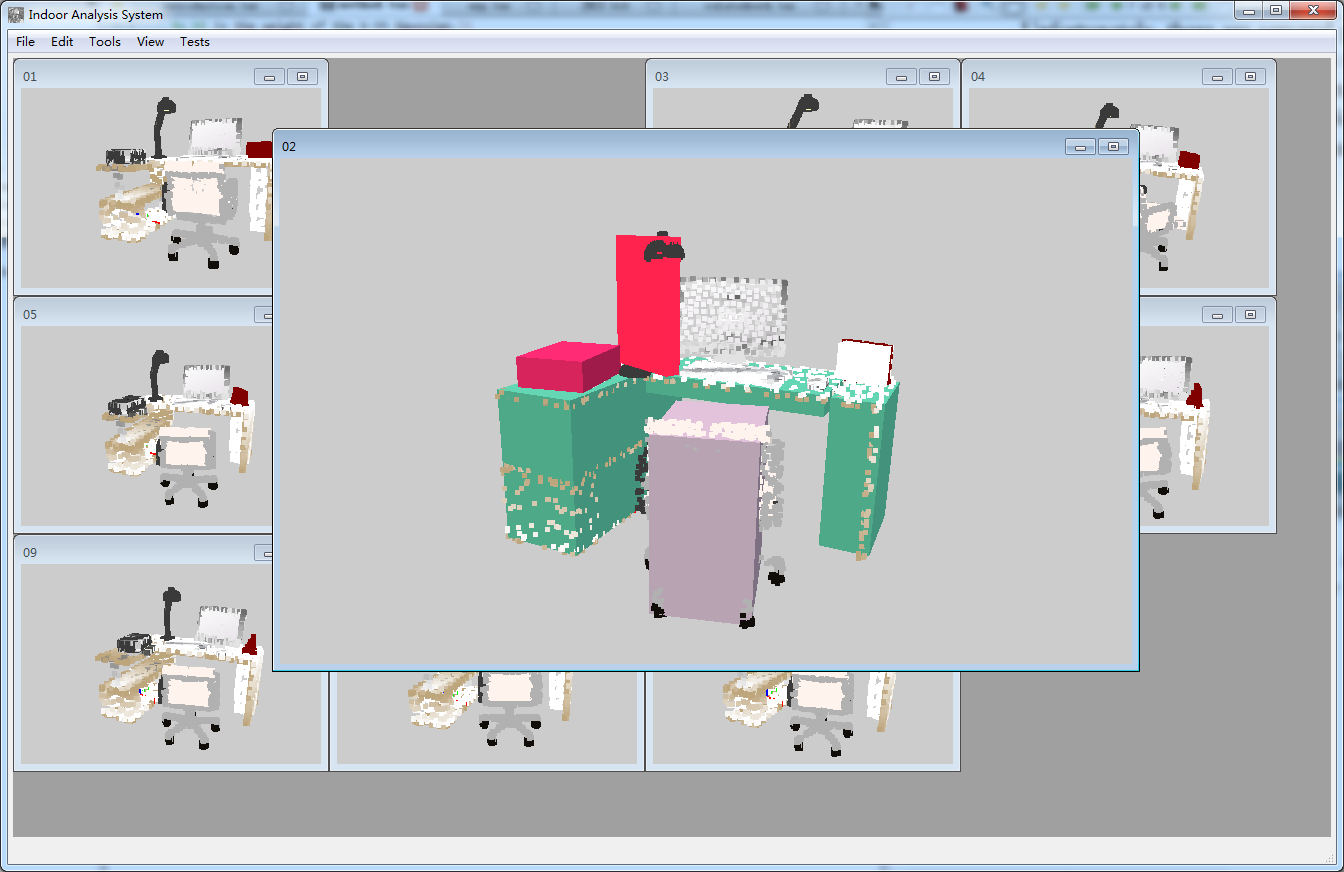
\includegraphics[width=.3\linewidth]{images/interact04.png}
	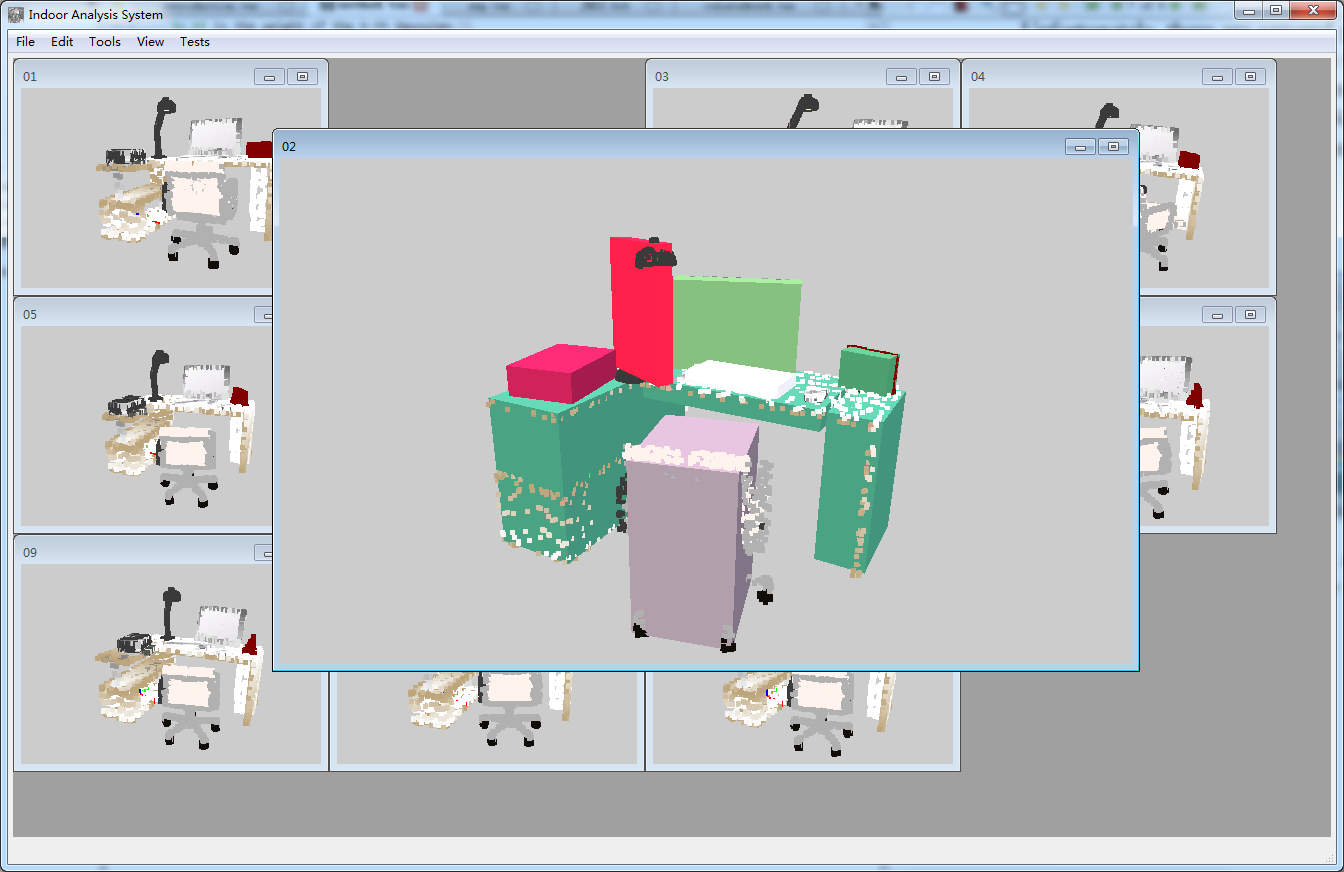
\includegraphics[width=.3\linewidth]{images/interact05.png}
	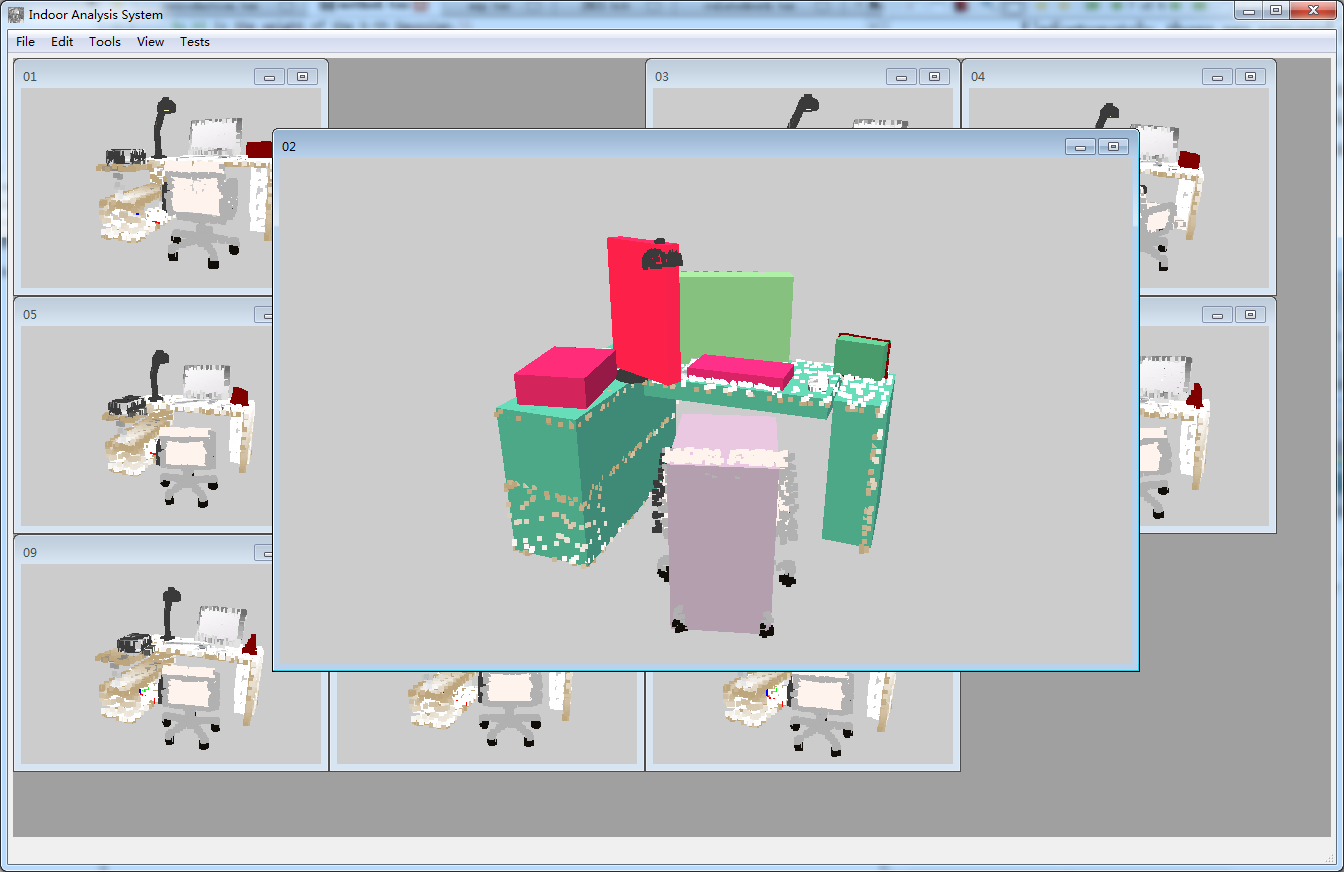
\includegraphics[width=.3\linewidth]{images/interact06.png}
	\caption{\label{fig:interact}
		From the first to the nineth, the nine images show the procedure of interaction:
		the user pick one point set and place boxes in it to indicate the layout for this point set. The box in white is the box currently under editing. The boxes in other colors are boxes placed to represent object layouts. One color represent one object. The interaction allows multiple boxes to represent same object.(e.g. the desk is represented by three boxes in same color)}
\end{figure}
These two paremeters are difficult to be initialized without semantic prior, but with the input of the users we can naturally initialize the $N$ as the number of different color label and the ${K_n}$ as 
\begin{equation}
\label{equ:K_n}
K_n=\frac{V_n}{\sum V_n}K_{all}
\end{equation}
in which the $V_n$ represent the total volume of the boxes in the $n^{th}$ color and the $K_{all}$ is initialized as $K_{all}=\frac{median(I_m)}{2}$ and $\{I_m\}$ are point numbers of $M$ input point sets. This is an emperical choice borrowed from \cite{Evangelidis2014}.\\
The expectation maximizaton framework is easily converged to a local optimal. To cope with this problem we further use this layout (boxes) from interaction as a soft constraint to guide the optimization and constrain the shape of generated object model. Such constraint is enforced by simply altering the posterior probability $\alpha_{mik}$ as\\
\begin{equation}
\label{equ:alteralpha}
\alpha_{mik}^*=\frac{\alpha_{mik}\beta_{mik}}{\sum_{i,k}\alpha_{mik}\beta_{mik}}
\end{equation}
where the $\beta_{mik}$ is the prior probability according to the boxes. It is defined as:\\
\begin{equation}
\beta_{mik}=\left\{
\begin{array}{rcl}
1& &\pmb v_{mi} \in B_n\\
\exp(-\frac{\min_{\pmb v_{mj}}|| \pmb v_{mi} - \pmb v_{mj} ||_2^2  )}{L})& &\pmb v_{mi} \notin B_n~and~\pmb v_{mj} \in B_n\\
\end{array} \right.
\end{equation}
where the $B_n$ is a point set that is enclosed by the boxes used to represent the layout of $n^{th}$ object. The $k^{th}$ Gaussian model is predefined to be one of the Gaussians used to represent $n^{th}$ object. $\min_{v_{mj}}|| v_{mi} - v_{mj} ||_2^2$ is actually the squared euclidean distance from point $v_{mi}$ to the point set $B_n$, as we define the distance from a point to a point set as the minimum distance from the point to any point inside the point set. $L$ here is a constant number with $L=2r^2$, and $r$ is the meadian of the radius of input point sets. The radius of a input point set is half of length of diagnonal line of its axis aligned bounding box.   
\begin{figure}[htb]
	\centering
	\includegraphics[width=\linewidth]{images/localoptimal/localoptimal}
	\caption{\label{fig:localoptimal}This figure shows an example result when converges to a local optimal. (a) is the result of segmentation of this local optimal. (b) is the final centroids of latent model. It shows that from top to down the 2nd and 3rd object model both include part of the table and part of the chair.}
\end{figure}
This alteration on posterior probability is only done with the probability related to the $m^{th}$ point set that have the mannual input layout (the boxes) in it. This alteration can help prevent the optimization from converging to a local optimal as in Figure~\ref{fig:localoptimal}. The result from the Figure~\ref{fig:localoptimal} have the same input and initialization with the result from Figure~\ref{fig:teaser}, but it doesn't use the posterior alteration as a soft constraint.


	\section{Algorithms and Implementation Details}
\label{sec:imp}
In this section, we summarize the entire algorithm and explain the implemented details.\\ 
\subsection{Algorithm}
Based on our formulation in section \ref{sec:method}, our algorithm can be summarized as in Algorithm \ref{alg:jrcs}.
\begin{algorithm}[htb]
	\caption{Joint Registration and Co-segmentation (JRCS)}
	\label{alg:jrcs}
	\textbf{Input:}~~\\
	$\{V_m\}$:$M$ input 3D point sets\\
	$\Theta^0$:Initial parameters~~\\
	$\{\beta_{ik}\}_{m}$:layout based prior\\
	\textbf{Output:}~~\\
	$\Theta^q$:Final parameters~~
	\begin{enumerate}
		\item $q\leftarrow1$
		\item \textbf{repeat}
		\item E-step: Use $\Theta^{q-1}$ to estimate $\alpha_{mik}^q$ according to (\ref{equ:estep}) ( (\ref{equ:bestep}) if use bilateral formulation)
		\item alter $\alpha_{mik}^q$ with $\{\beta_{ik}\}_{m}$ according to (\ref{equ:alteralpha})
		\item M-step-a: Use $\alpha^q_{mik}$, $\pmb x^{q-1}_k$ to estimate $\{R_{mn}^q\}$ and $\{\pmb t_{mn}^q\}$ according to (\ref{equ:updateR})(\ref{equ:updatet})
		\item M-step-b: Use $\alpha^q_{mik}$, $\{R_{mn}^q\}$ and $\{t_{mn}^q\}$ to other parameters for Gaussian models according to (\ref{equ:updatexk})(\ref{equ:updatesigma})(\ref{equ:updatepk})(\ref{equ:updatey})  ( and (\ref{equ:updatefk})(\ref{equ:updatefsigma}) if use bilateral formulation)
		\item $q \leftarrow q+1$
		\item \textbf{until} Convergence
		\item \textbf{return} $\Theta^q$
	\end{enumerate}
\end{algorithm}
\subsection{Implementation Details}
\textbf{Initialization of $\Theta$}:\\
We first determine the total number of Gaussian model $K_{all}$ as we explained in subsection \ref{sec:imp:interact}. We set $p_k=\frac{1}{\sum K_n}$ which means each Gaussian model have the same weight at the beginning. We seperate the Gaussian models into $N$ groups to represent $N$ objects. Each group has $K_n$ Gaussian models based on (\ref{equ:K_n}). $\{\pmb x_k\}_n$ are Gaussian centroids of $n^{th}$ group and they are initialized as a random positions uniformally distributed on the surface of a sphere. The radius of the sphere is chosen as the median of the radius of the input point sets $r$. The center of the $n^{th}$ spheres is $c_n=(0,0,z_n)$, where $z_n\in \{-(N-1)r,-(N-3)r,...,(N-1)r\}$. This means that the object models are vertically arranged in latent space as shown in Figure~\ref{fig:teaser}(m)(n) and in Figure~\ref{fig:localoptimal}(b).We choose vertical arrangement for groups of object merely for the convenience of visualization. We choose the sphere as the initial shape so that we can initialize all the $R_{mn}$ to identity matrix. For the $\pmb t_{mn}$ we initialize them as $\pmb t_{mn}=- \pmb c_n$ so that all the object model starting with position at origin point when they are transformed to the space of each input set. However, if the $m^{th}$ input point set has the manually placed layout, we treat the associated $\pmb t_{mn}$ differently. For this case we have:
\begin{equation}
\label{equ:initt}
\pmb t_{mn}=\frac{\sum_{\pmb v_{mi} \in B_n}\pmb v_{mi}}{N(B_n)}-\pmb c_n
\end{equation}
where $N(B_n)$ is the number of element in $B_n$ and $B_n$ is the point set that is enclosed by the mannual input layout (boxes). 
\subsection{Hot Intervention Machinism}
Our current implementation of optimization is quite slow (fail to converge in interative time) especially when the point numbers inside each input point set are large and it is possible for our optimization to stuck in a local optimal, requiring the guide from the mannual input. As a compensation for these drawbacks. We implement a hot intervention machinism, allowing the mannaul input take effect even after the optimization has started. Theoretically, this is possible due to the i.i.d assumption. 
This assumption makes it possible for the calculation of posterior probability being independent for each input point set. Even after the optimization is started, we can still allow the user to add more layouts for other point sets and the program can do the same alteration as (\ref{equ:alteralpha}) in the next iteration. The Figure~\ref{fig:hi} shows how the users can use the hot intervention machinism within our tool.
\begin{figure}[htb]
	\centering
	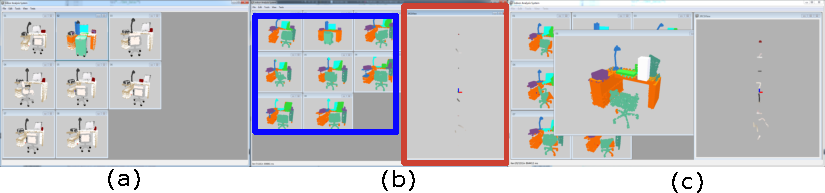
\includegraphics[width=\linewidth]{images/hotintervention/hi}
	\caption{\label{fig:hi}This figure shows the hot intervention machinism. (a) is the input point sets with mannually placed layout in 2rd point set. (b) shows that from the region highlighted by blue rectangle the user can see the instant result of segmentation and from the region highlighted by the red rectangle the user can see the space of object model(the shape of the centroids of the Gaussian models). (c) shows that the user picks another input point set and add more boxes targeting the incorrect segmentation to further guide the optimization.}
\end{figure}
 
	\section{Experiment and Discussion}
\subsection{Evaluation for Co-segmentation on Synthetic Data}
\begin{figure}[htb]
	\centering
	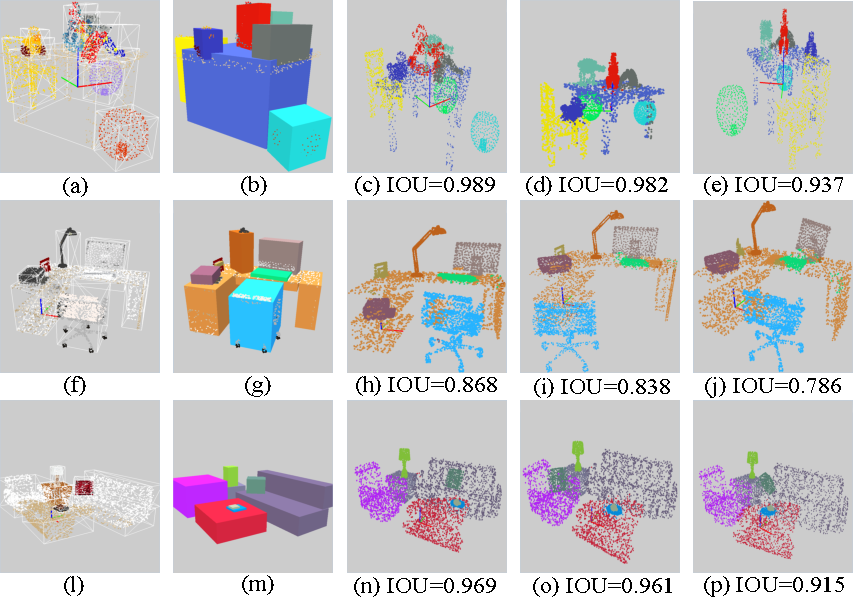
\includegraphics[width=0.8\linewidth]{images/seg/seg}
	\caption{\label{fig:seg}Three rows in the figure shows segmentation evaluations on three groups of synthetic data (child table, office desk, living room). Each group of data have 13 point sets. The first column are examples of point sets for each group of data. The second column are mannual placed layout for each group of data. The $3^{rd}$ column shows the segmentation result with maximum IOU scores in the groups. The $4^{th}$ column shows the segmentation result with median IOU scores in the groups. The $5^{th}$ column shows the segmentation result with minimum IOU scores in the groups.}
\end{figure}
From the perspective of co-segmentation, we evaluate our algorithm on synthetic data of indoor scenes. To estimate the power of the algorithm we only input layout for one point set in each group for initialization and do not use the hot intervention mechanism. For numercial \cxj{->numerical} estimation, we calculate the intersection over union (IOU) scores for the result segmentation against ground-truth segmentation. We generate three group of synthetic point sets and each group have 13 point sets as inputs. The Figure~\ref{fig:seg} shows the result of the evalution \cxj{->evaluation}.


From the evaluation, we want to discuss one interesting observation:\\
%
For all three groups, the point set with highest IOU score is not the same as the point set equiped with manually placed layout.In other words , the point sets from the $3^{rd}$ column in Figure~\ref{fig:seg} are not the same point sets from $2^{nd}$. In the first group of data (dataset of child table in Figure~\ref{fig:seg}), the segmentation result of the point set with layout is even the second worst in the sense of IOU score. We believe this is because that the manually placed layout is not accurate respecting to point-wise segmentation. At early iterations of the optimization, the alteration in (\ref{equ:alteralpha}) can serve as a soft constraint to help \mdf{constraining} the shape of object, but in the final iterations the alteration will obstruct the further improvement of segmentation for the correspondent point set. 



\subsection{Evaluation for Joint Registration on Synthetic Data}
From the perspective of joint registration, we evaluate the result by transfering \cxj{->transferring} the point cloud of objects  to each input point set based on result $\{\phi_{mn}\}$ and calculating the average distance from a point to its true correspondent point for each input point set.  We use this average distance as fitness error to evaluate the registration quality respect to each input set.
Table~\ref{tab:regerror} shows the result of this evaluation.
\begin{table}
\centering
\begin{tabular}{c c c c}
Dataset & Maximum Error & Median Error & Minimum Error \\
\hline
Child Table & 0.0715 & 0.0112 & 4.91e-005 \\   
Office Desk & 0.189  & 0.0618 & 0.00518 \\
Living Room & 0.132  & 0.0563 & 0.0301\\
\end{tabular}
\caption{Error for registration of the same three groups of data in Figure~\ref{fig:seg} The unit of these numbers is 1 meter}
\label{tab:regerror}
\end{table}
For this evaluation we want to discusss \cxj{->discuss} that:\\
We find that even the input set with high IOU scores in segmentation can result in high fitness error. We believe this is due to the symmetric and near-symmetric objects in the scene. For symmetric objects, even the registration is correct the distance from a point to its true correspondent point can be high, since the rotation in registration result can be different from the one we use to generate this synthetic data. For near-symmetric objects, the registration often stuck in a local optimal and result in high IOU score but high fitness error.
\subsection{Test On Real Data}
\begin{figure*}[htb]
	\centering
	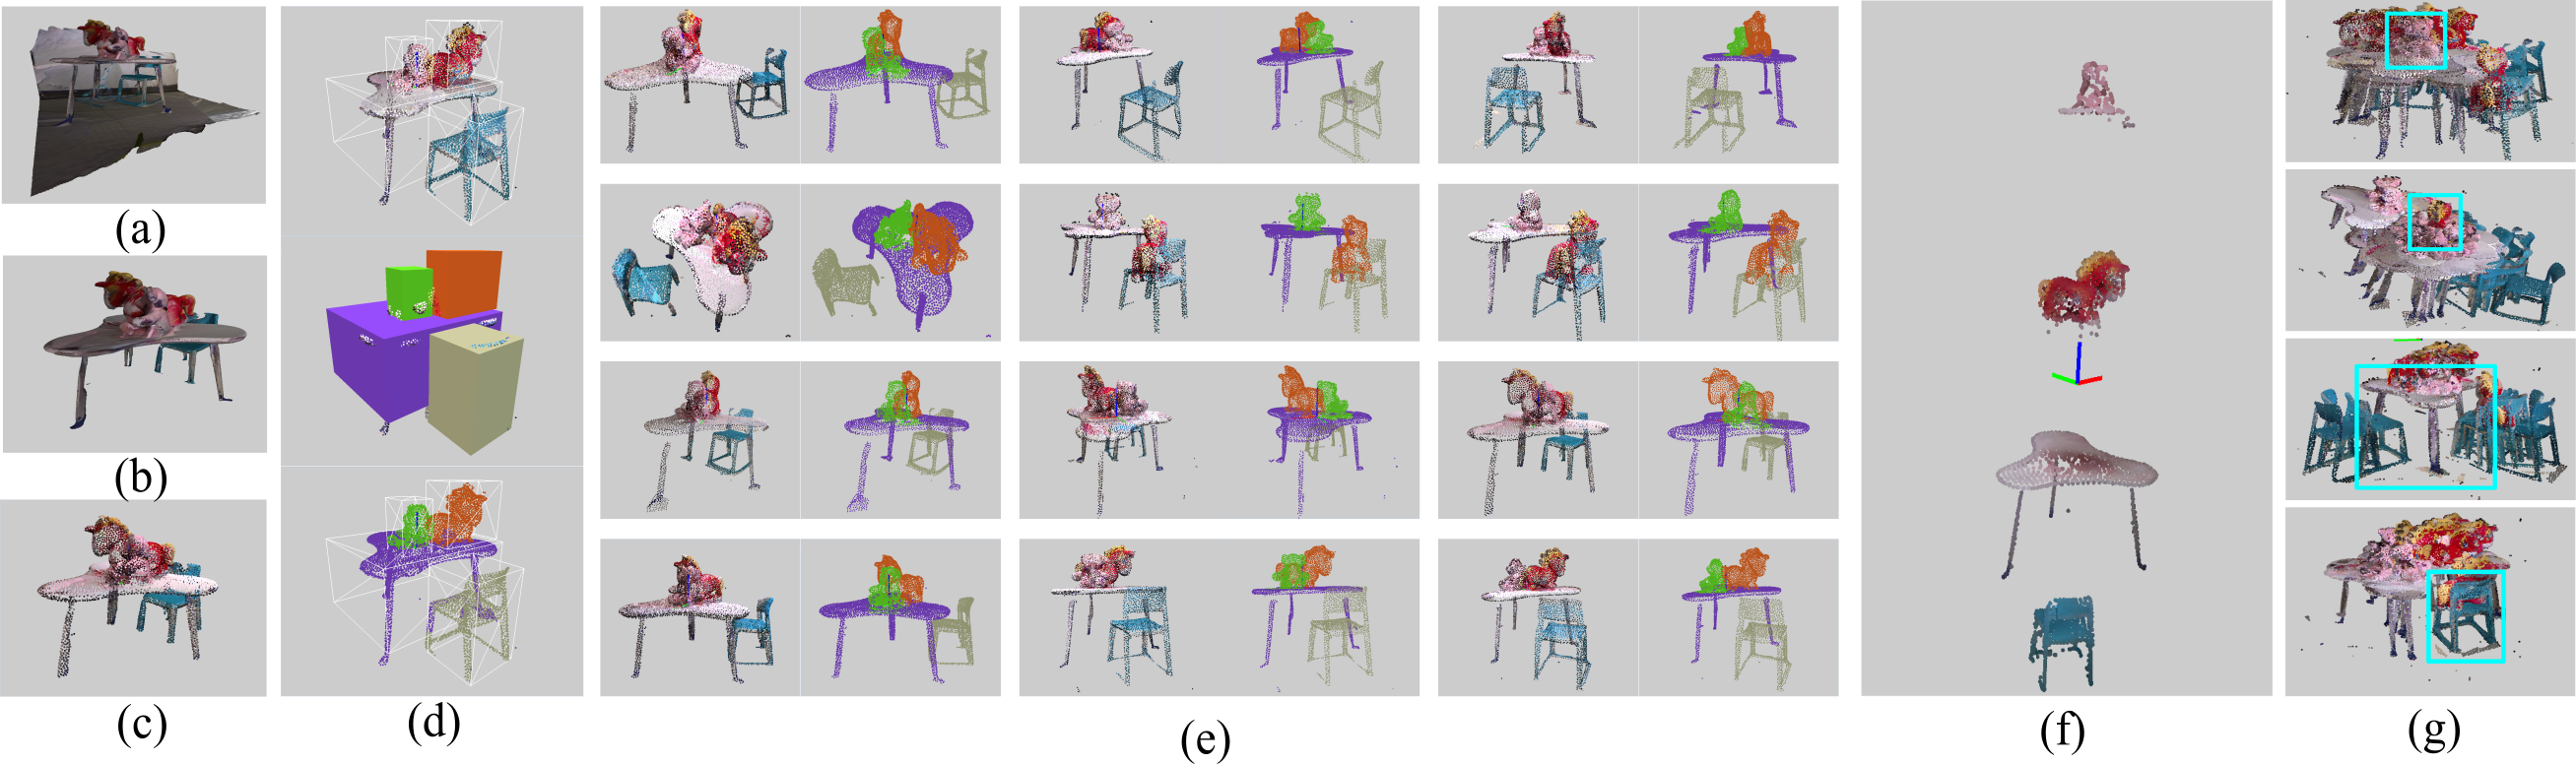
\includegraphics[width=\linewidth]{images/realdata/realdata}
	\caption{\label{fig:realdata}This figure shows our test on a real data. (a) shows how we capture real data with method in \cite{VXH} (b) shows result after we remove walls and floors by plane fitting (c) shows we generate point set with method in \cite{PossionSampling}. (d) shows the first input point set, the input layout on it and its segmentation result. (e) shows all other pairs of input point sets and corresponding segmentation result. (f) shows the final Gaussian centroids from top to down correpondent to different objects (g) verifys the registration result by aligning input point sets respecting to each object. The light blue rectangle highlights the object that is aligned together. }
\end{figure*}
To capture real data we employ the method of \cite{VXH} and use plane fitting to remove walls and floors. We then transfer the mesh into point set with the sampling process from \cite{PossionSampling}.
We test our algorithm on the sampled point sets. Figure~{\ref{fig:realdata}} shows the complete result of our test. On real data, there are noised color, shape distortion, partial scanning and outliers as they are highlighted in Figure~\ref{fig:challenge}. 
\begin{figure}
	\centering
	\includegraphics[width=\linewidth]{images/challenge/challenge}
	\caption{\label{fig:challenge}This figure highlights the common challenges on real data.}
\end{figure}
From Figure~\ref{fig:realdata}(e), we can see that all input point sets are partitioned into objects. From the Figure~\ref{fig:realdata}(g), we can verifys \cxj{->verify} that the object from each input set are aligned together by the result transformation.  
\subsection{Limitations and Future Work}
The biggest problem holding us back is the time performance of current implementation of our tool.  Due to i.i.d. assumption most calculation of our algorithm can actually be parallelized. We plan to implement a new version on GPU cluster so that we can explore more potentials of our algorithm, for example,Try to integrate semantic feature vectors (generated by neural networks) into it and try it on a scene of larger scale like \cite{GOGMA}. As advocated in the recent work of \cite{AGM}, it may be a good idea to do the joint registration and co-segmentation with hierarchical GMM representation when applyed to scenes on a larger scale. 
	
	%-------------------------------------------------------------------------
	%\bibliographystyle{eg-alpha}
	\bibliographystyle{eg-alpha-doi}
	\bibliography{JRCS}
	%-------------------------------------------------------------------------
\end{document}